\documentclass[12pt]{article}

\usepackage{amsmath}
\usepackage{amssymb}
\usepackage{graphicx}
\usepackage{full page}

\begin{document}
\title{Dynamic Aperture and Dynamic Binning}
\author{Alexander Heckett}
\maketitle
\begin{abstract}
Traditional, astronomical, photometric methods of computing star intensities and calculating uncertainties in measurements lead to unnecessarily large error bars. Dynamic Aperture and Dynamic Binning are clever ways of reducing error both in the computation of star intensities and in their analysis that allow for smaller fluctuations in star brightness to be detected. These methods are explored conceptually, grounded algorithmically, and implemented with dramatic results. When used in sync, these two methods frequently halve error bars.
\end{abstract}
\tableofcontents
\section{Background}
\subsection{Summary}
\indent \indent Over the last week, I have been working on a program that could significantly aid in the detection of fluctuations of astronomical objects, such as the identification of exoplanet transits, quasar and black hole monitoring, or any other varying electromagnetic source. The results are pleasingly dramatic, while the computation time required to attain them is only a few seconds on even quite slow computers. Furthermore, they are currently implemented in Python, which is a programming language known for ease of programming but a slow runtime, further illustrating the lack of computation power required to run these procedures.
\subsection{Terminology}
\indent \indent Before lunging into the details of the project, a quick review of background topics is appropriate. Lightcurves are simple plots of the emissions of an electromagnetic source over time. The number of photons (or any other unit) is recorded on the y-axis, while the time (equivalently, frame number) is marked on the x-axis. Before we can conclude anything about an object's behavior, we must know something about how certain our measurements are. For instance, there is no detectable difference between an intensity of 100,000 and 100,050 photons if we are only certain of our measurements to within 10,000. However, calculating an uncertainty can be very difficult, so it is often preferred to use the dataset itself to deduce this. We partition up our dataset into chunks within which we believe our object does not vary. We then conclude that all fluctuation within such a chunk (formally known as a \textit{bin} or a \textit{block}) must be noise due to our detection mechanism. We assume that any one of those measurements must have been somewhere between the minimum and the maximum of that bin, but can say no more about them with much confidence. The difference between the maximum and the minimum is known as the height of the \textit{error bar}.
\newline
\indent Inherent in this procedure is a fundamental tradeoff: accuracy versus confidence. We can choose to have very large bins, in which case we are virtually \textit{certain} a measurement will lie between the minimum and the maximum, but because we have a large number of frames in our block, we lose the fine detail of the structure of the lightcurve. On the complete contrary, we can chose to have tiny bins, in which case all fine detail is preserved, but we have little faith that a measurement will lie between the minimum and maximum, because we have only shown this to be true for a small number of frames. Picking what bin size in-between these two opposites to go with is one task that drastically effects what changes in intensity are detected by a program.
\section{Concepts}
\subsection{Existing Methods}
\indent \indent At this point, we are prepared to hear the traditional route taken for computing the intensity at any moment of a source in the sky, as well as the partitioning up of the lightcurve of such intensities into bins. The intensity of a star (or any other object) is defined to be the sum over all pixels inside a circle centered somewhere in the source that completely encompasses the star, as well as a good deal of the space around that object. Optionally, at very little computational cost, this can be made more accurate by taking some sample of pure space (no additional stars in this region) near our star as representative of the local background noise, whose average brightness per pixel can be taken off the sum previously found. This method does indeed sum over the entire star, but it also sums over a good deal of empty space. I shall call this \textit{Static Aperture}, because the aperture of the star (the region of space we sum over) does not change from frame to frame.
\newline
\indent The most common method for finding the partitioning to use is to take blocks of a fixed size. This rigidly defines the appropriate place to put the tradeoff between accuracy and confidence, ignoring any opportunities to, say, move the boundaries of these blocks around by just a few frames in order to dodge large spikes, or even to optimize the heights of these blocks depending on the local shape of the lightcurve. I will call this \textit{Static Binning}, because the bins are all of the same size.
\subsection{New Ideas}
\indent \indent At this stage, we are in a position to make some cuts to the error bar heights, allowing finer detail to be seen in these lightcurves. Let's start by changing Static Aperture to a new method for computing intensity, \textit{Dynamic Aperture}. When computing intensities via Dynamic Aperture, at every frame we calculate the exact boundary of the star, pixel by pixel, and sum over that region, hence the name ``Dynamic.`` Since we are summing over fewer pixels, we are introducing less uncertainty, and hence reducing the error of our measurements. 
\newline
\indent Another improvement we can make is to use \textit{Dynamic Binning}, as opposed to Static Binning, in which we customize our bins to have different sizes from each other. This allows for the program to make optimizations that would otherwise be impossible, hence reducing the observed error bars, even if we are not improving the lightcurve itself. 
\section{Algorithms}
\subsection{Dynamic Aperture}
\indent \indent Now, we must figure out a way to execute our plan. First, we need to attempt to implement a Dynamic Aperture. We wish to separate the bright star from the relatively dim background, so a good starting point would be to make this distinction precise. We dip into our pool of ``pure background`` to find the mean and standard deviation of the background pixels. Assuming that the brightness of background pixels follows a Gaussian distribution, we can use this to figure out what cutoff, say, $ \frac{1}{50} $ of the background is above. Once we have this cutoff, we go look inside our circle that the star must be completely contained in to figure out what pixels satisfy this requirement. The star can be assumed to be so bright that all pixels containing the star appear. As well, many unwanted, stray bright pixels will be included. The task at this point is to separate the star from the strays. While it is highly probable that \textit{some} background pixels will be included, it is \textit{extremely} improbable that they will all be connected. However, the star definitely will be in one piece. Therefore, all we have to do to find the star is to detect the largest contiguous block of extraordinarily bright pixels. This can be done by taking a pixel in our set of bright specks, exploring up, right, down, and left until we have traced out the patch of other bright specks it is connected to, and seeing if we have already found another patch with this many connected. If not, then set this to be our record. Of course, if a bright speck has already been visited, don't bother re-exploring that same patch again. At the end of this procedure, we will have the largest contiguous block of bright pixels together. This is how we define our star.
\subsection{Dynamic Binning}
\indent \indent Our task for executing Dynamic Binning is no easier. The first, and by far hardest, part of this task is to define what the word \textit{better} means. I define a better partitioning of a lightcurve to mean that we get more information about it, which in turn I define to mean a lower average standard deviation, weighted by the number of frames each bin has. However, since I only have error bar heights to work with, there is no point in talking about the standard deviation of the data directly. We can only infer the standard deviation of a bin given how tall the bar is and how many frames the block contains. How do we make this inference? First, we pre-compute the average heights of bars with a certain number of frames in them, given that the data we have has mean $ 0 $ and standard deviation $ 1 $, and save this as a .txt file for many different numbers of frames (in my case, I pre-computed $ 2 $ to $ 500 $). I'll call this function $ \zeta \left ( n \right ) $, where $ n $ is the number of frames we have in a bin. Then, we can use this .txt file to draw the conclusion that:
\begin{align}
\sigma & = \frac{h}{\zeta \left ( n \right )}
\end{align}
Where $ h $ is the height of our error bar, $ \sigma $ is the standard deviation of the data within our bin, and $ n $ is the size of our sample. Then plugging this formula into an average gives a metric for the ``badness`` of a collection of bins (the quantity which we will ask our program to minimize):
\begin{align}
b & \equiv \frac{\sum_{i} \left [ \frac{n h_{i}}{\zeta \left ( n_{i} \right )} \right ]}{\sum_{i} \left [ n_{i} \right ]}
\end{align}
Since $ \sum_{i} \left [ n_{i} \right ] $ is just the total number of frames we're analyzing, it doesn't make sense to divide by this constant, since $ b $ can be multiplied by any (positive) number to give an equally valid ``badness metric.`` This lets us define $ \tilde{b} $:
\begin{align}
\tilde{b} & \equiv \sum_{i} \left [ \frac{n h_{i}}{\zeta \left ( n_{i} \right )} \right ]
\end{align}
We have here a curious phenomenon. The badness of this collection of bins is a sum of ``badnesses`` for each bin:
\begin{align}
\tilde{b}_{i} & \equiv \frac{n h_{i}}{\zeta \left ( n_{i} \right )}
\end{align}
This convenience allows us to write an extremely speedy algorithm for finding the very best partitioning to use, as opposed to needing to check every different possibility, which would make this problem completely impossible computationally! We can handle this problem recursively. Let's say we know the best ways to partition the lightcurve up, starting at every place to the right of some given position. We also know the total ``badness`` of partitioning the lightcurve from that point on that way. Well, to find the best way to partition the lightcurve up from our given position, we just check the badness of the partitioning from the test location on, plus the little additional badness of the block we would need from our given ``root`` to the test location, compared to the best known solution (a long block stretching from our root to the very end of the lightcurve). Therefore, $ n $ items until the end of the lightcurve, it takes $ O \left ( n \right ) $ additional pieces of computation for every unit you go to the left. That makes this algorithm $ O \left ( n^{2} \right ) $. Compared to an exponential, $ O \left ( n^{2} \right ) $ looks pretty good!
\newline
\indent In fact, we're not even done. Our algorithm currently finds the best possible partitioning. However, we can place constraints on this program that both speed it up (by requiring it to look over fewer possibilities) and place bounds on the types of partitionings it can output. Firstly, we can set an upper limit on how large a bin we will accept. If we are expecting fluctuations on the order of, say, 500 frames, we can accept bins no larger than, perhaps, 750 frames, because blocks that are longer will run the risk of hiding important changes. The main purpose of this limit, however, is really to speed up the program. Since we only need to look for junctions a fixed distance forward, our $ O \left ( n^{2} \right ) $ algorithm becomes $ O \left ( n \right ) $! Granted, a better way of writing this would probably be $ O \left ( n m \right ) $, where $ m $ is the maximum number of frames a block can contain. This $ n $ dependence is the best that could possibly be conceived. For a quick thought-experiment style proof, we could make some frame arbitrarily large, which can make a given partitioning arbitrarily unprofitable compared to one in which that frame is in a bin of size $ 2 $ (if we have an odd length lightcurve, not every bin can have size $ 2 $, thus there is at least one location that, if we ``inflate`` its value, can be shown to be in a sub-optimal bin). Thus, we have to at least look at every value in the lightcurve, which means that any algorithm attempting to find the best partitioning must be at least $ O \left ( n \right ) $. 
\newline
\indent We can equally well set a lower limit on the number of frames in a bin. This gives us an upper bound on the probability that a measurement will leak outside our error bars, which is given by the formula:
\begin{align}
p & = \frac{2}{n + 1}
\end{align}
Thus, we have two algorithms, Dynamic Aperture and Dynamic Binning, which reduce our uncertainty in star brightness measurements.
\newline
\section{Results}
\subsection{Statistics}
\indent \indent I have implemented these two methods in Python. Now we get to examine their results. For my dataset (1,712 frames of PG 1718+481), I have taken a Dynamic Aperture P-value of 0.05, a Dynamic Binning unspecified maximum length, and a Dynamic Binning maximum P-value of 0.2. The average length of a bin, weighted by the number of frames in each bin, is $ 37.85 $. This indicates that the program often found it profitable to make larger bins with higher sizes to allow for larger $ \zeta $. The smallest bin my program generated is of size $ 10 $, meaning that at least once my program maxed out the limit on bin sizes (on the lower end, at least). One (weighted) quarter of my bin sizes are at or below $ 15 $, while the median bin size is $ 23 $ (again, weighted by the number of frames a bin contains). Since $ 23 < 37.85 $, we have reason to believe that the distribution of weighted bin sizes is skewed to the right. Three quarters of the weighted bin sizes are below 43, while the largest bin size is 132. If we set the static block size to $ 38 $ for a side-by-side comparison of performance, we see that using Dynamic Blocking with the same average (weighted) bin size as Static Blocking reduces the average error bar heights by a factor of $ 1.255 $. It also reduces $ \tilde{b} $ by a factor of $ 1.158 $. Using Dynamic Aperture further reduces the weighted average of error bar heights by a factor of $ 1.554 $, coming out to a grand total of a $ 1.951 $ factor reduction! This large reduction factor has been purchased at only a couple of seconds of computation time, making Dynamic Aperture in junction with Dynamic Blocking an effective way of reducing the uncertainty in star intensity measurements. 
\subsection{Figures}
\indent \indent As a second form of result, we can examine some plots and visual displays of our program. To demonstrate Dynamic Aperture visually, Figure 1 is a sample ``star`` detected by my code. 
\begin{figure}[h]
\begin{center}

\includegraphics[scale = 10]{small}
\caption{A blown up image of a star, with pixels closer to red representing more light, and pixels closer to blue representing less. The blue ring is the border of the star as found by the Dynamic Aperture program.}
\end{center}
\end{figure}
Everything inside the blue border is the star. The border itself consists of the closest pixels to the star that aren't included as part of the source. Judging by eye, it looks as though our algorithm is doing a good job! For Figure 2, I have taken my test dataset and plotted a lightcurve of one star in the photograph. 
\begin{figure}[p]
\begin{center}
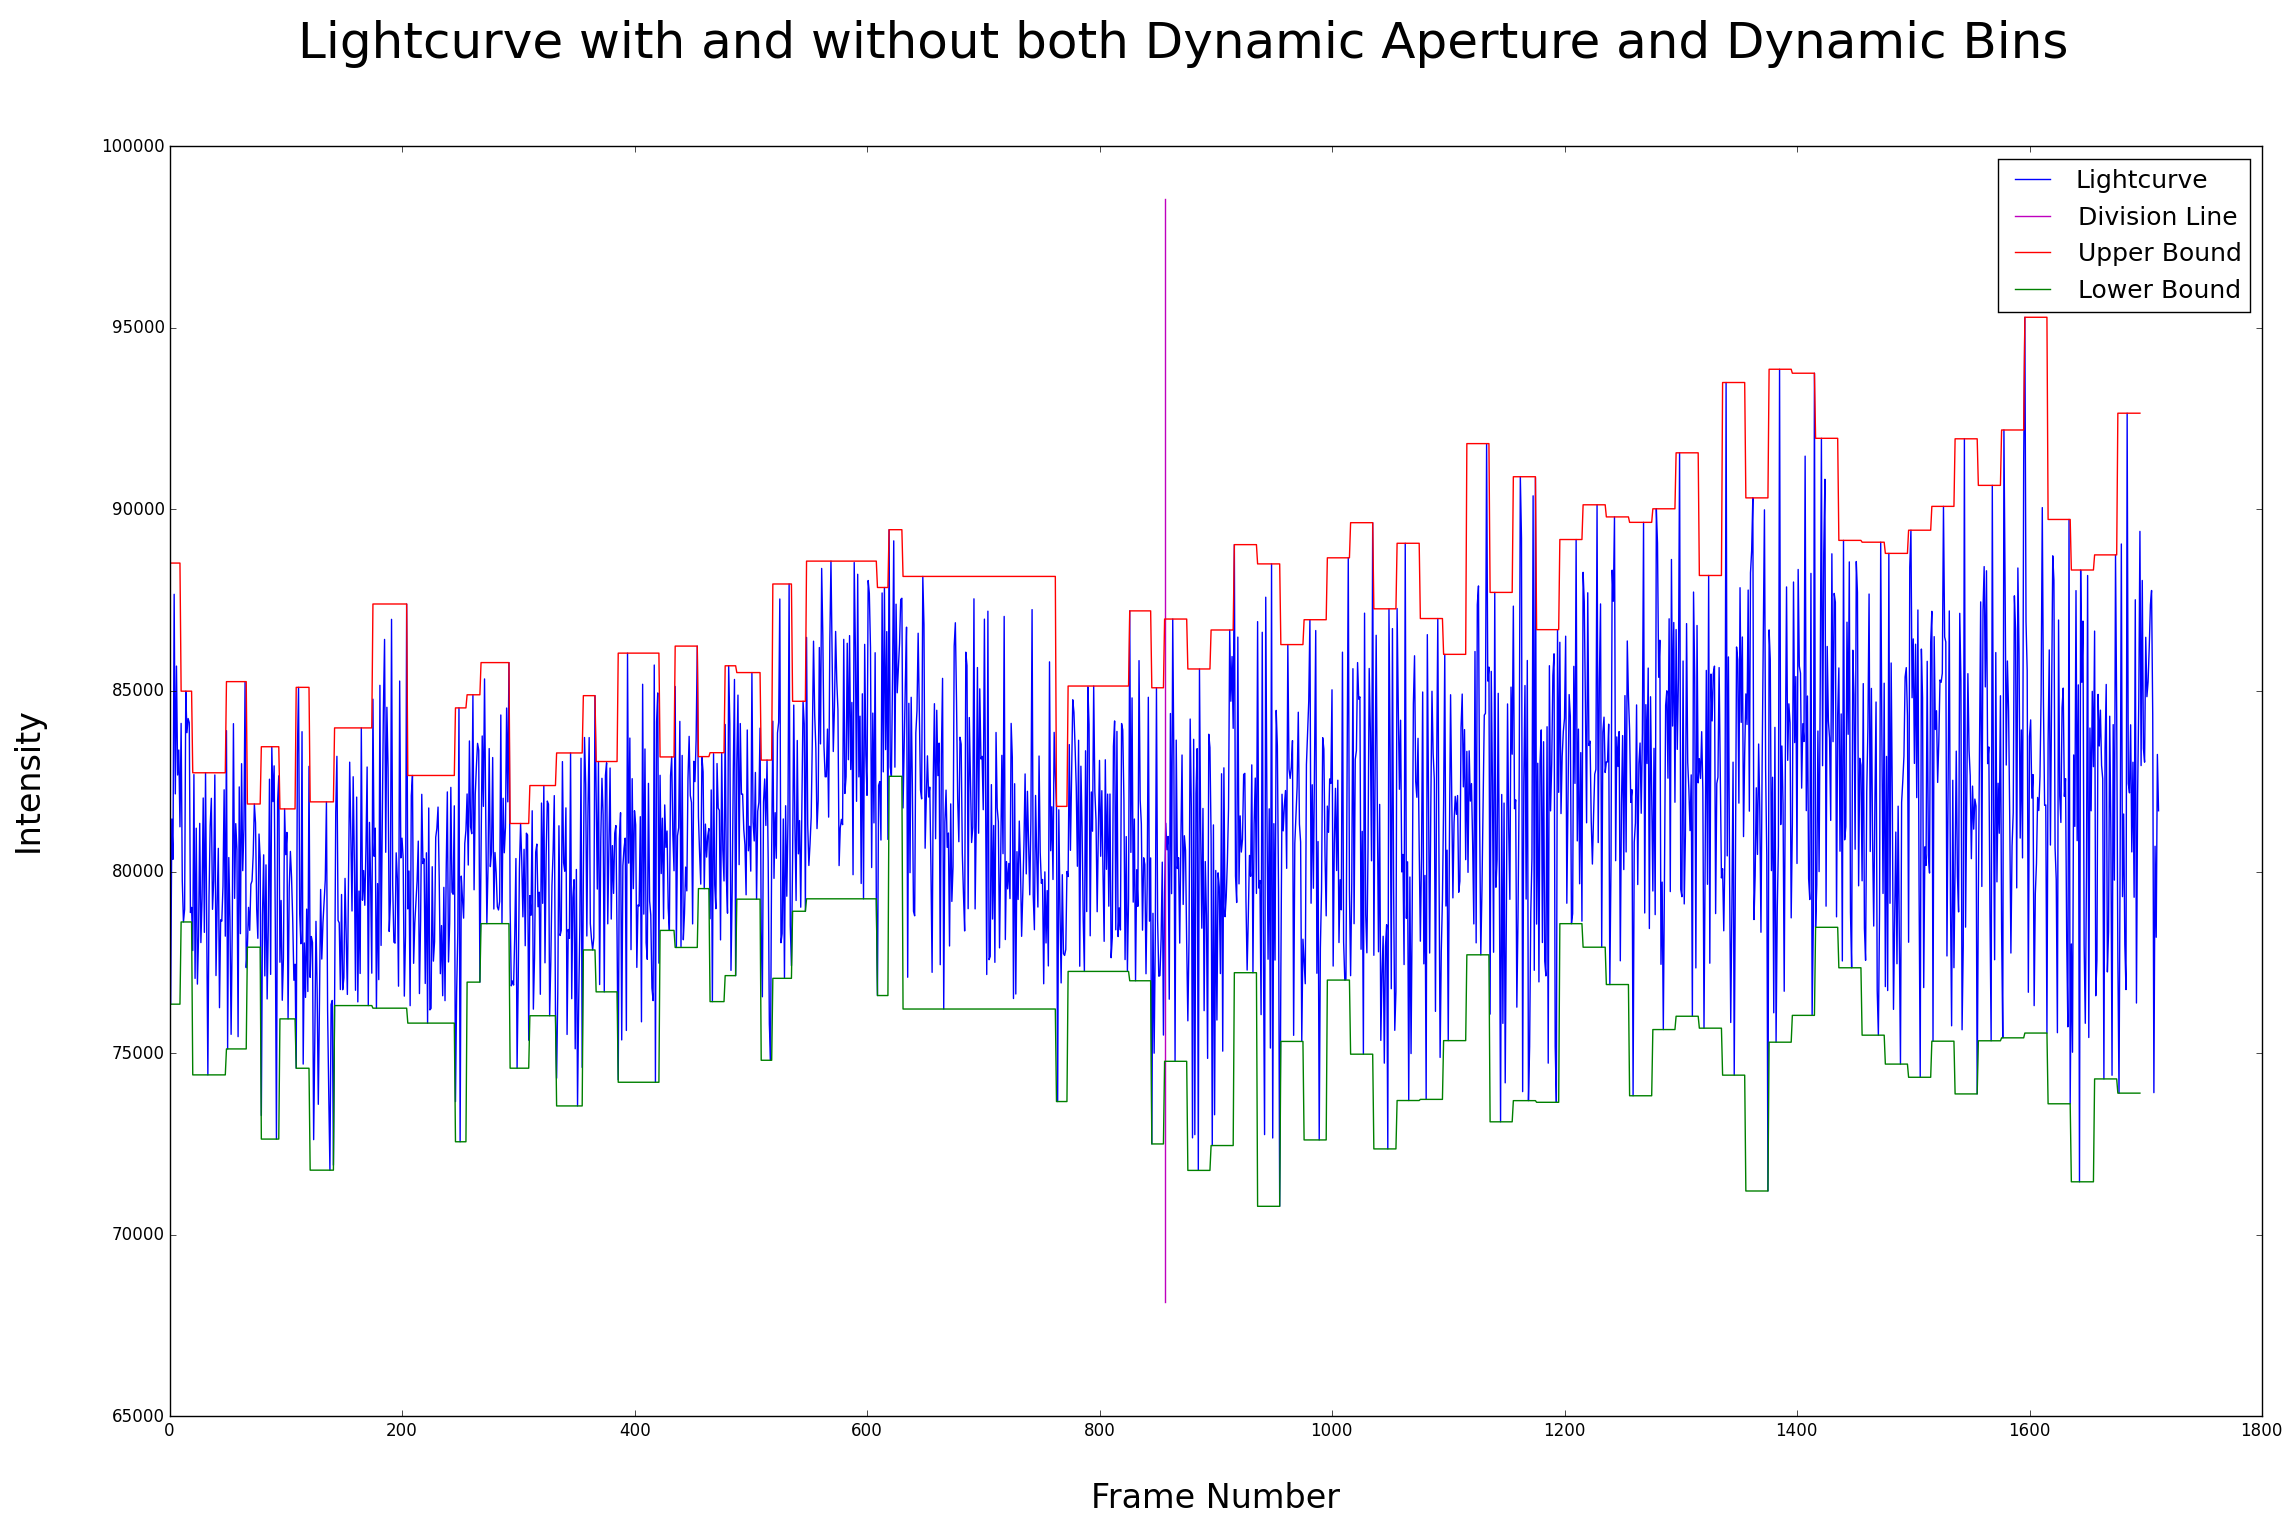
\includegraphics[scale = 0.3]{lightcurve_split}
\caption{The lightcurve of a star throughout 1712 consecutive frames. The left half of the image has been processed by both Dynamic Aperture and Dynamic Binning, while the right half uses conventional methods.}
\end{center}
\end{figure}
On the left of the purple dividing line, I have both used Dynamic Aperture to reduce the fluctuation of the lightcurve and Dynamic Binning to get the best bound on the data. On the right, I have used neither. Clearly, these techniques reduce the size of the error bars! We can also demonstrate the reduction in error bar height by plotting them as two different curves on the same graph, as is done in Figures 3 through 6 for different sizes of the Static Bins.
\begin{figure}[p]
\begin{center}
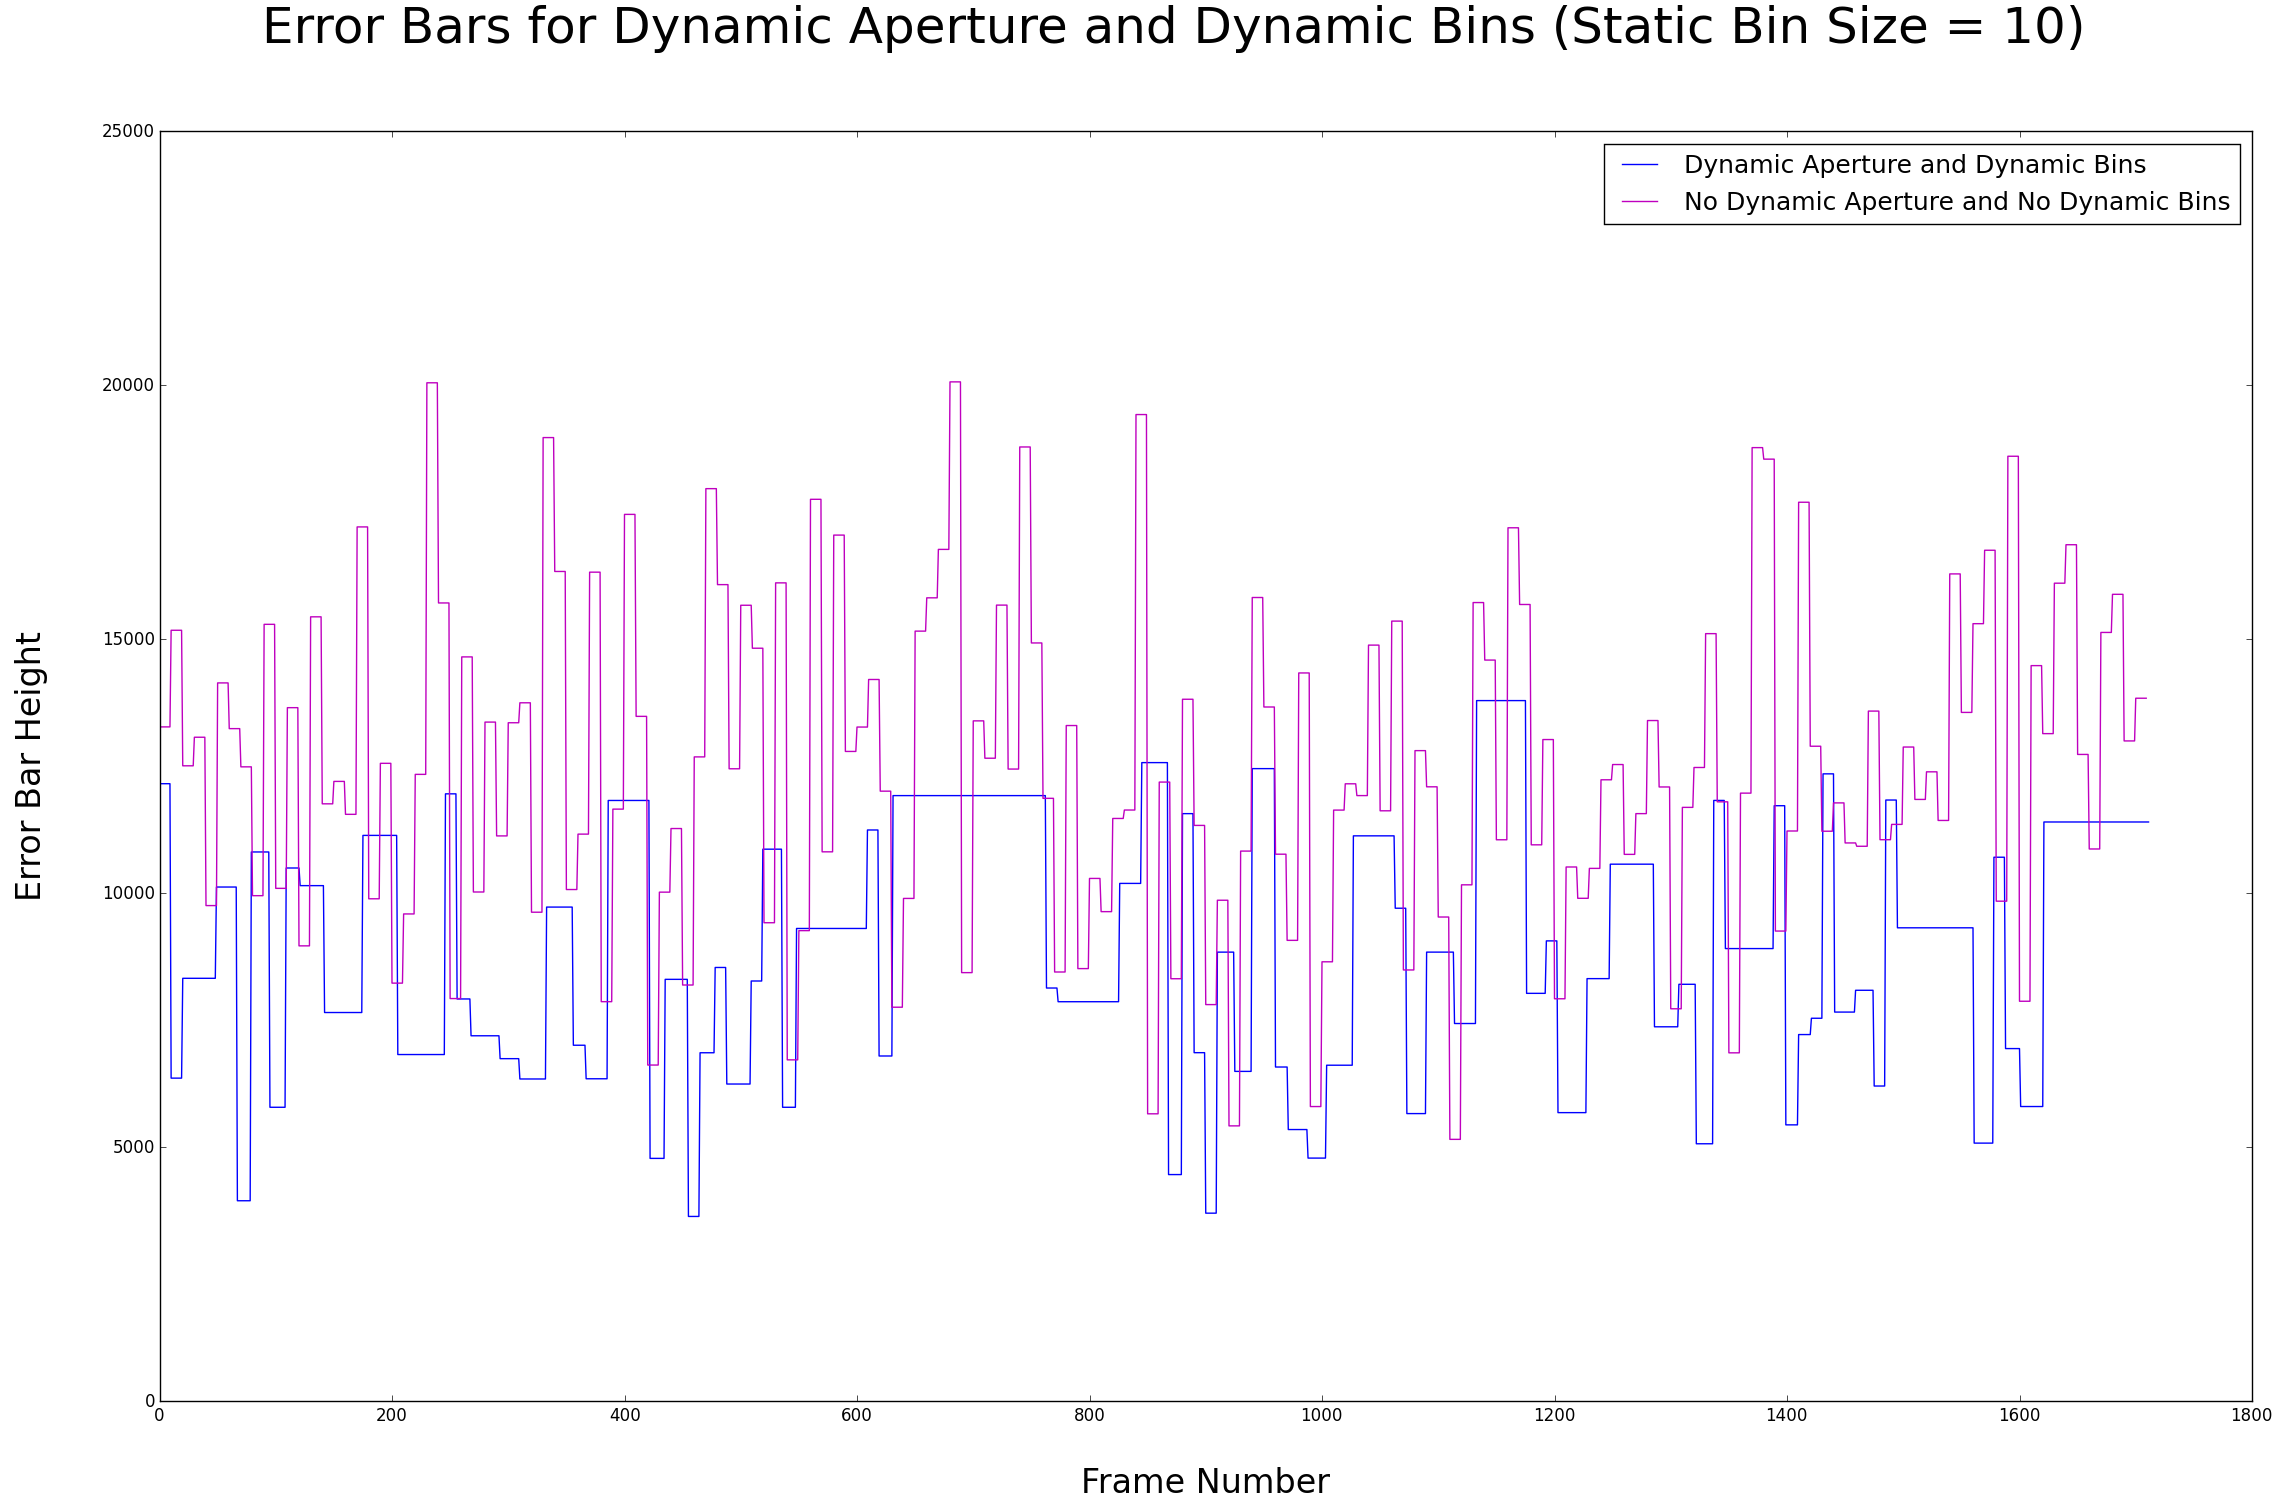
\includegraphics[scale = 0.3]{10.png}
\caption{Dynamic Aperture and Dynamic Blocking alongside neither. The Static Bin Size is 10.}
\end{center}
\end{figure}
\begin{figure}[p]
\begin{center}
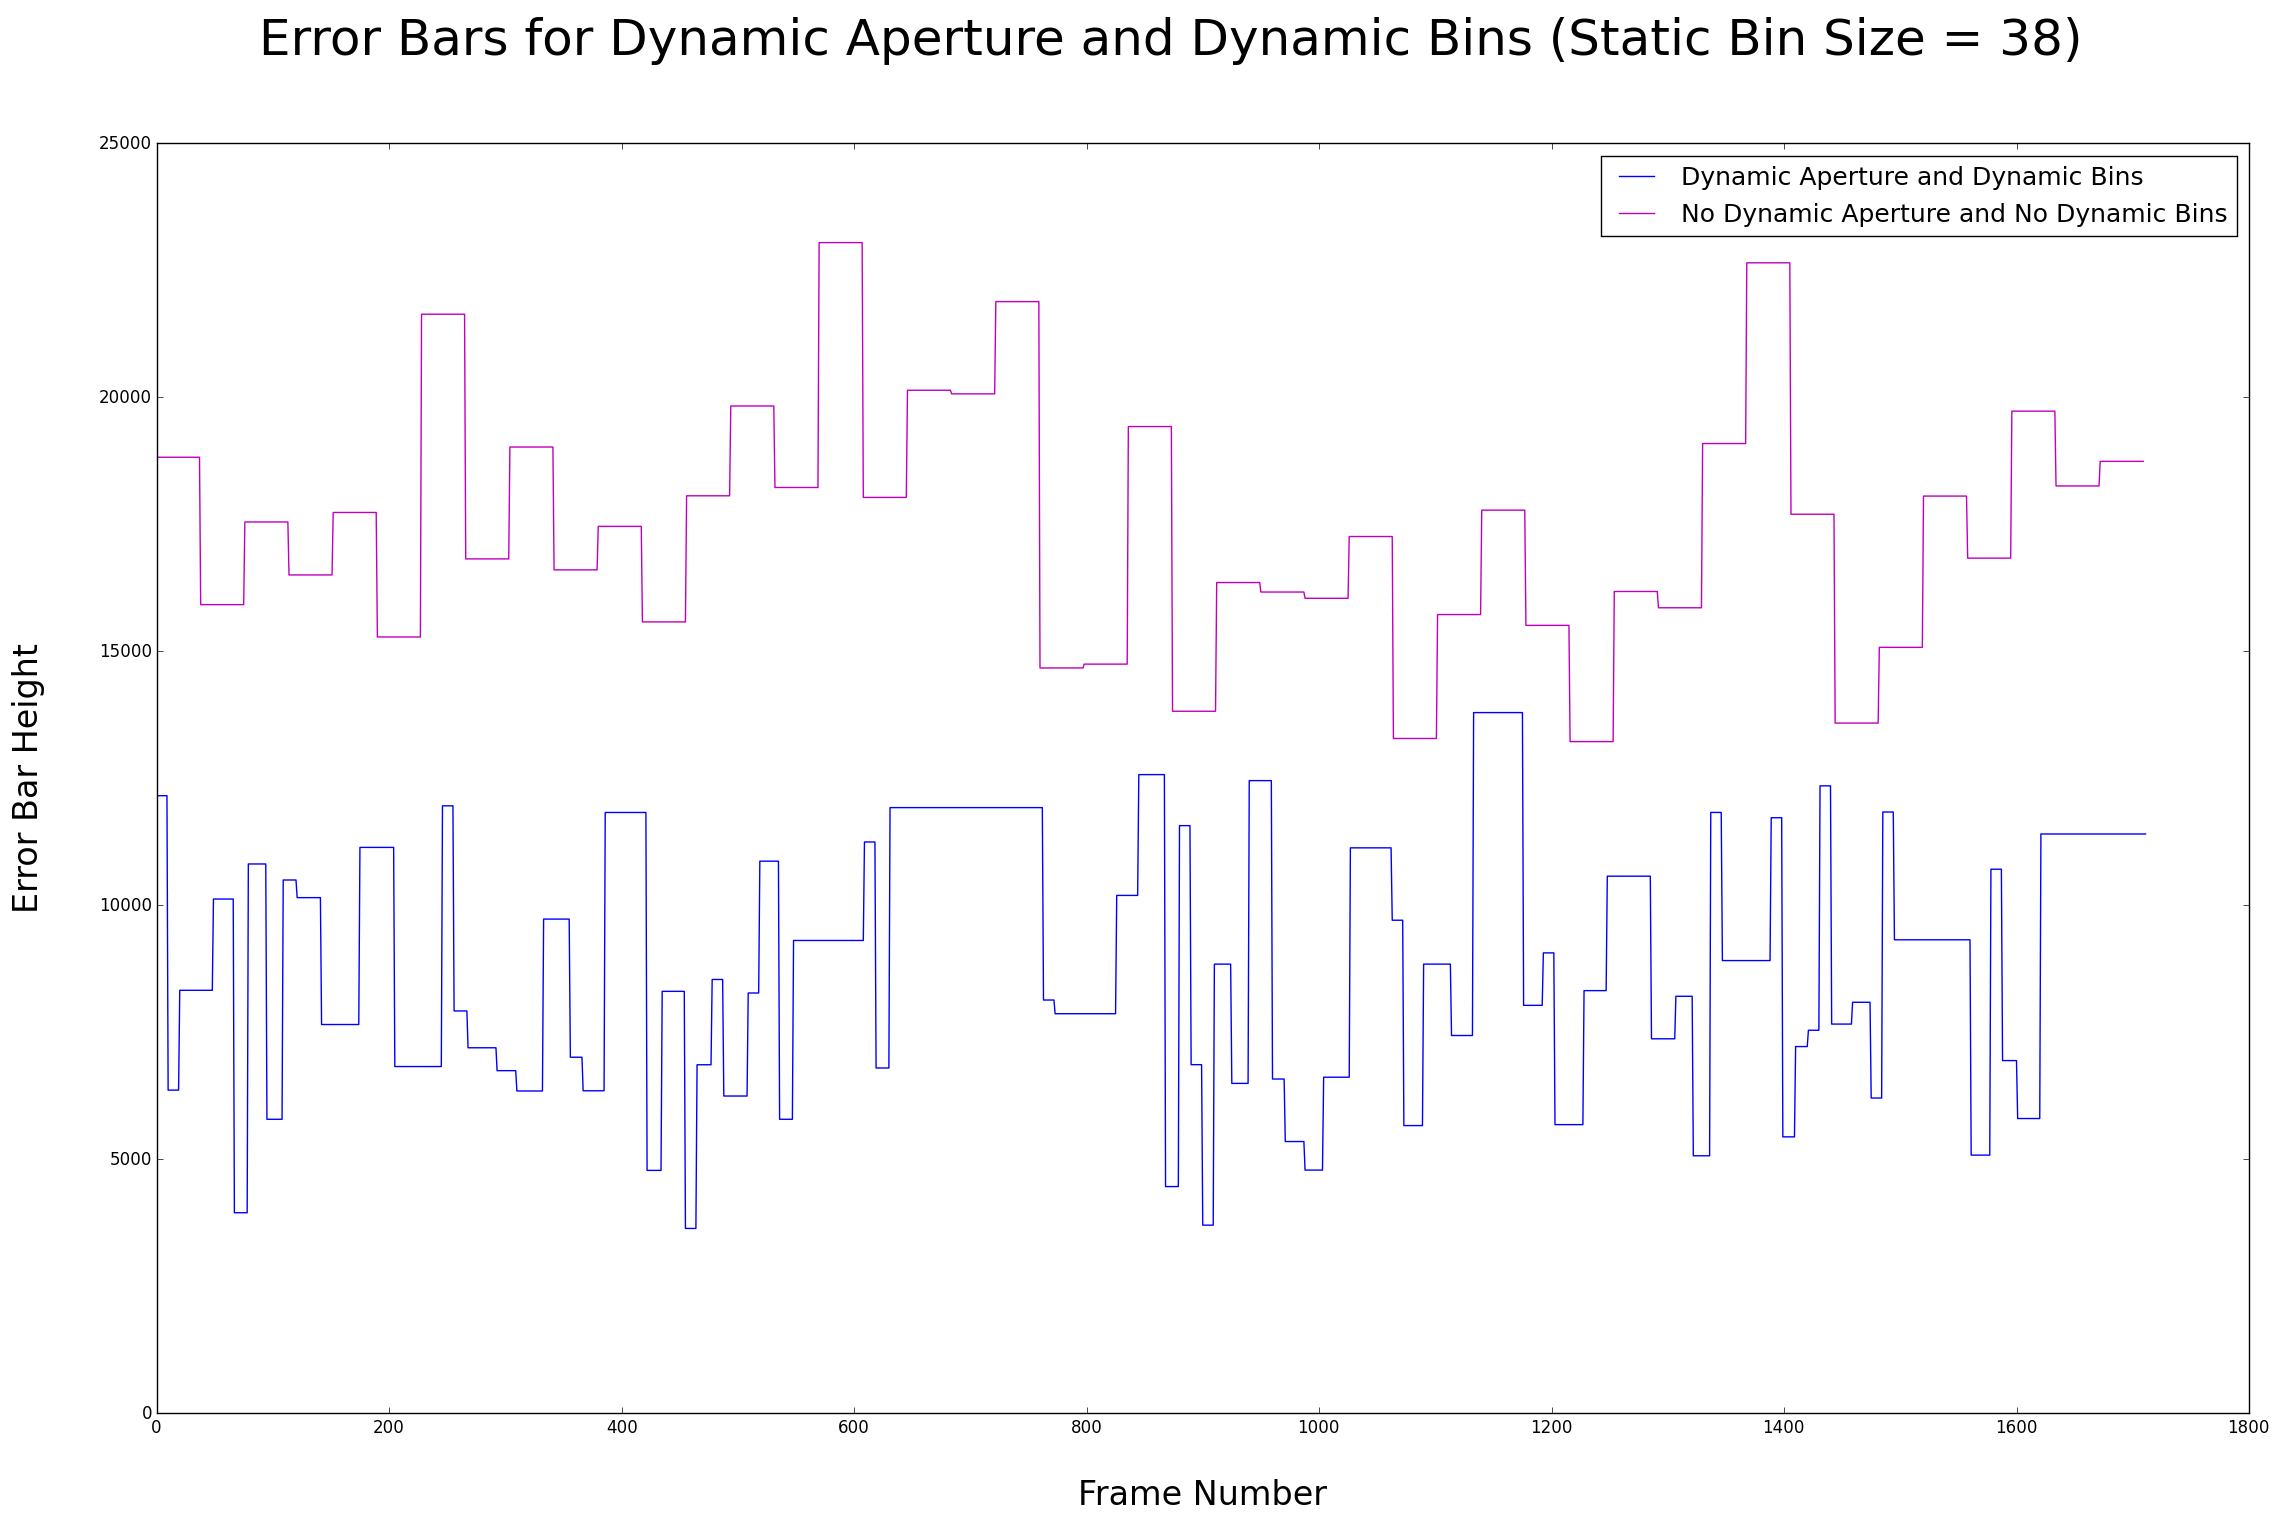
\includegraphics[scale = 0.3]{38.png}
\caption{Dynamic Aperture and Dynamic Blocking alongside neither. The Static Bin Size is 38, which is also the weighted average bin size of Dynamic Aperture. Thus, we have a fair comparison.}
\end{center}
\end{figure}
\begin{figure}[p]
\begin{center}
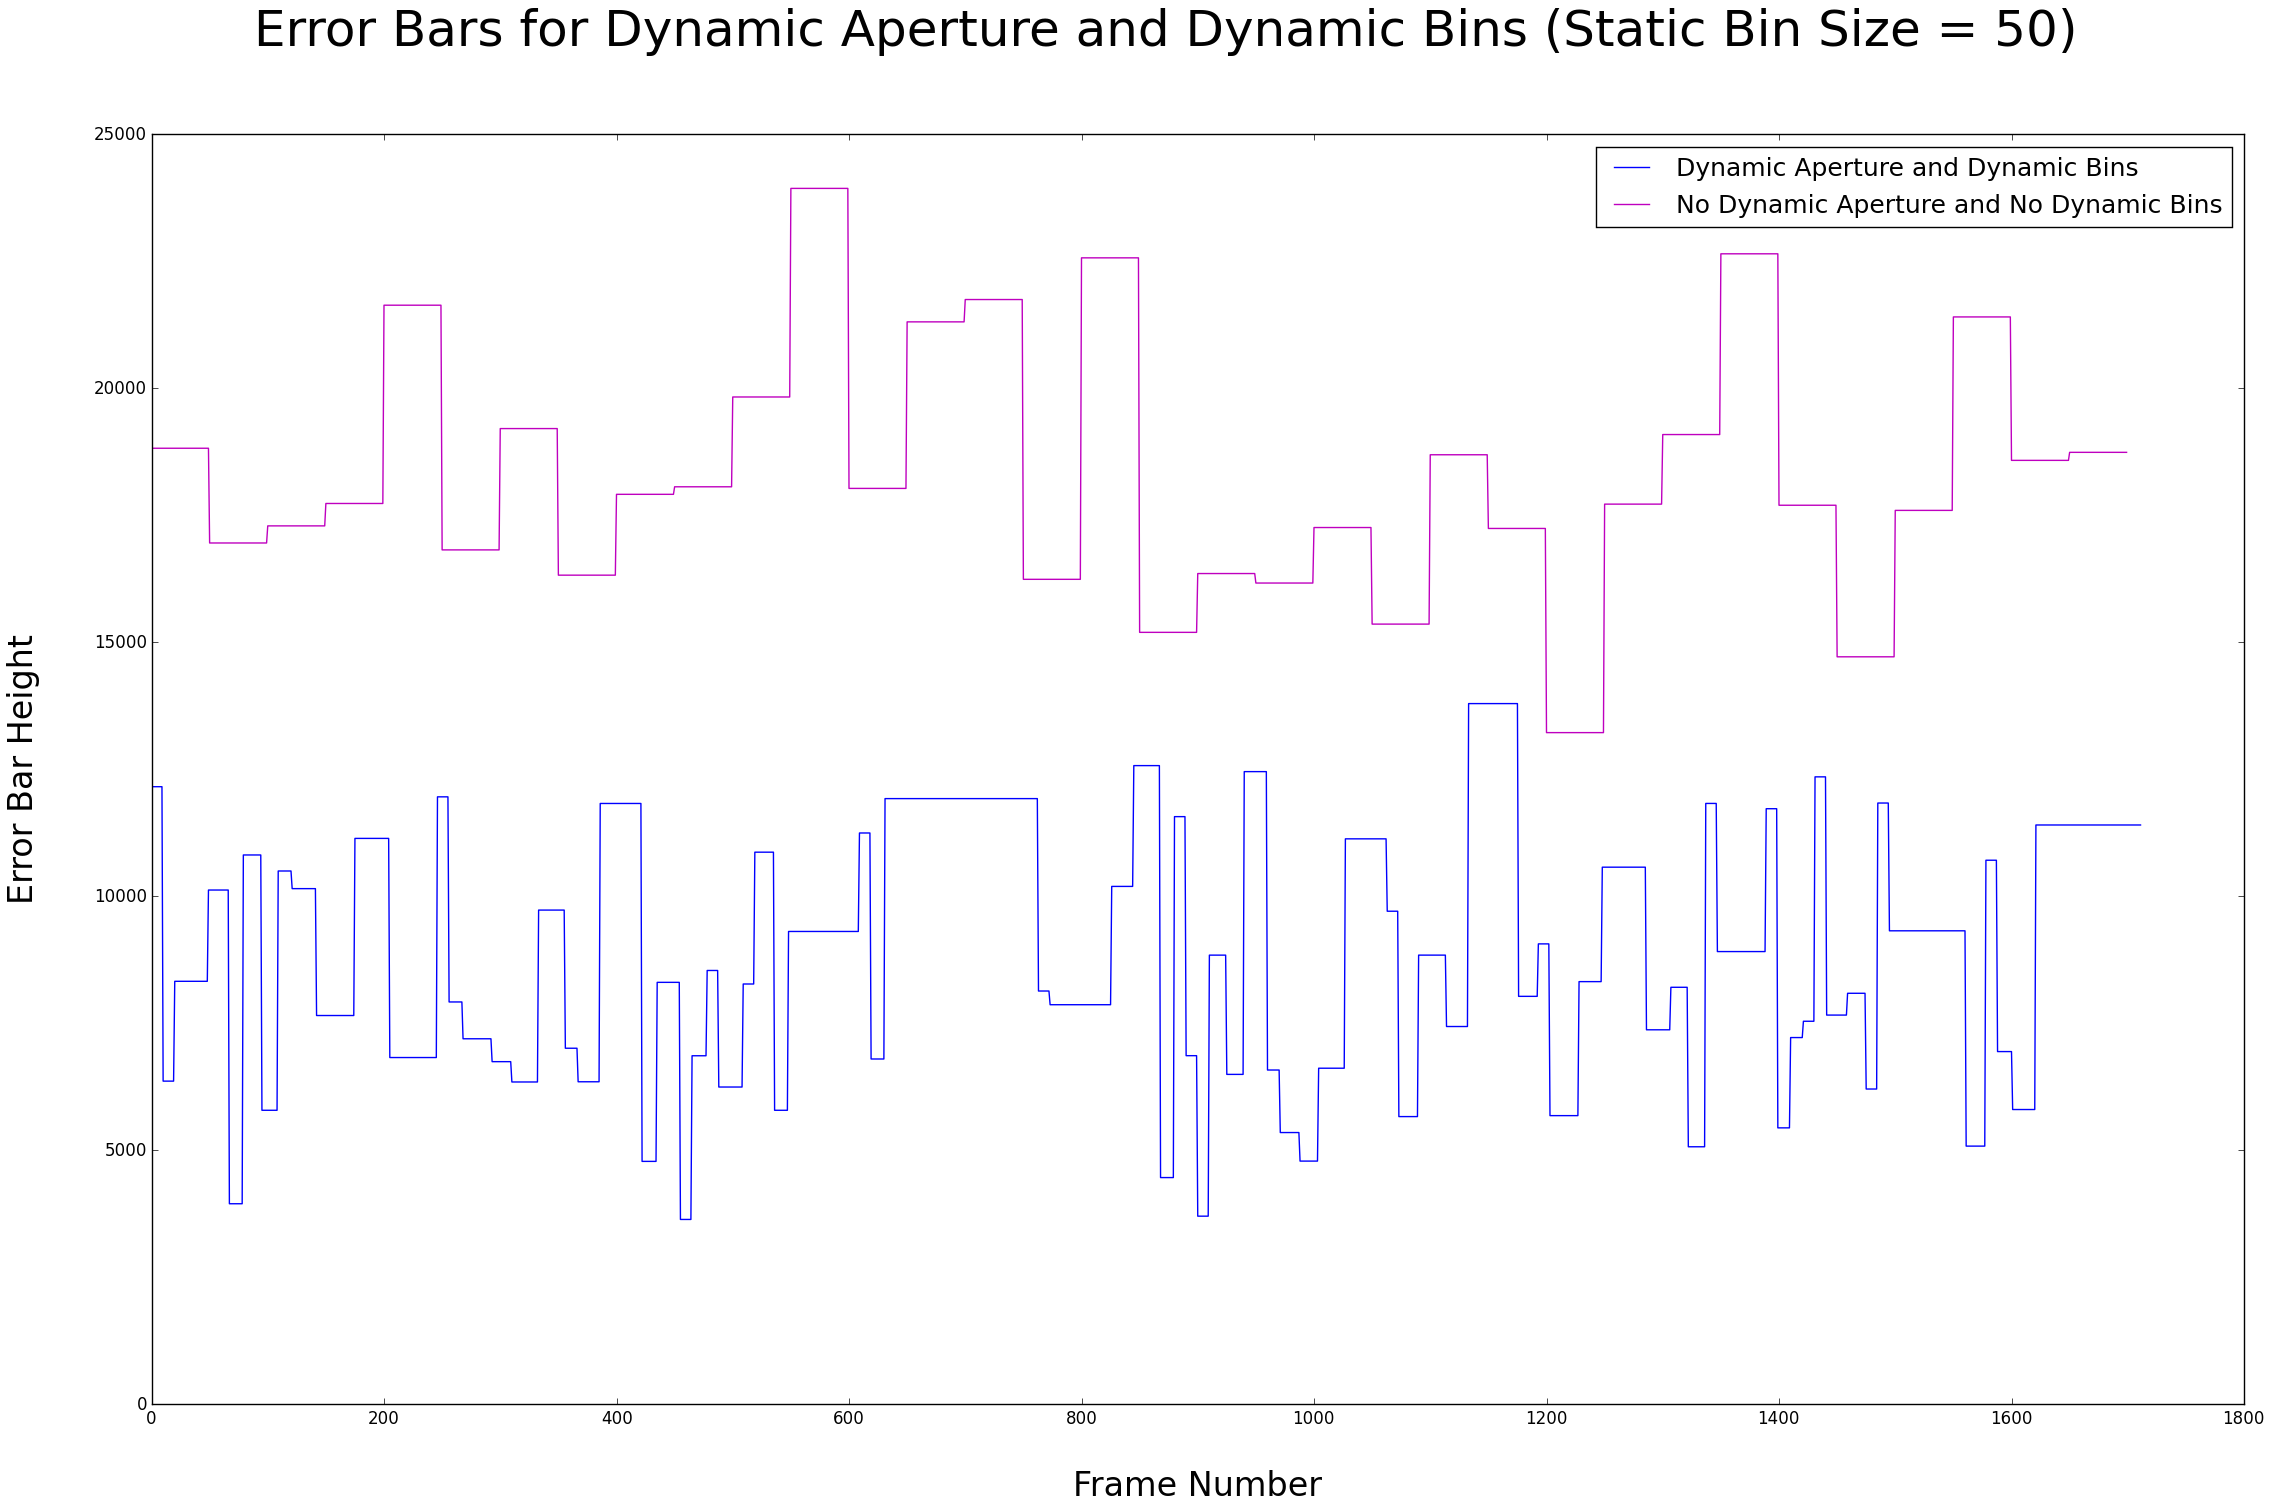
\includegraphics[scale = 0.3]{50.png}
\caption{Dynamic Aperture and Dynamic Blocking alongside neither. The Static Bin Size is 50.}
\end{center}
\end{figure}
\begin{figure}[p]
\begin{center}
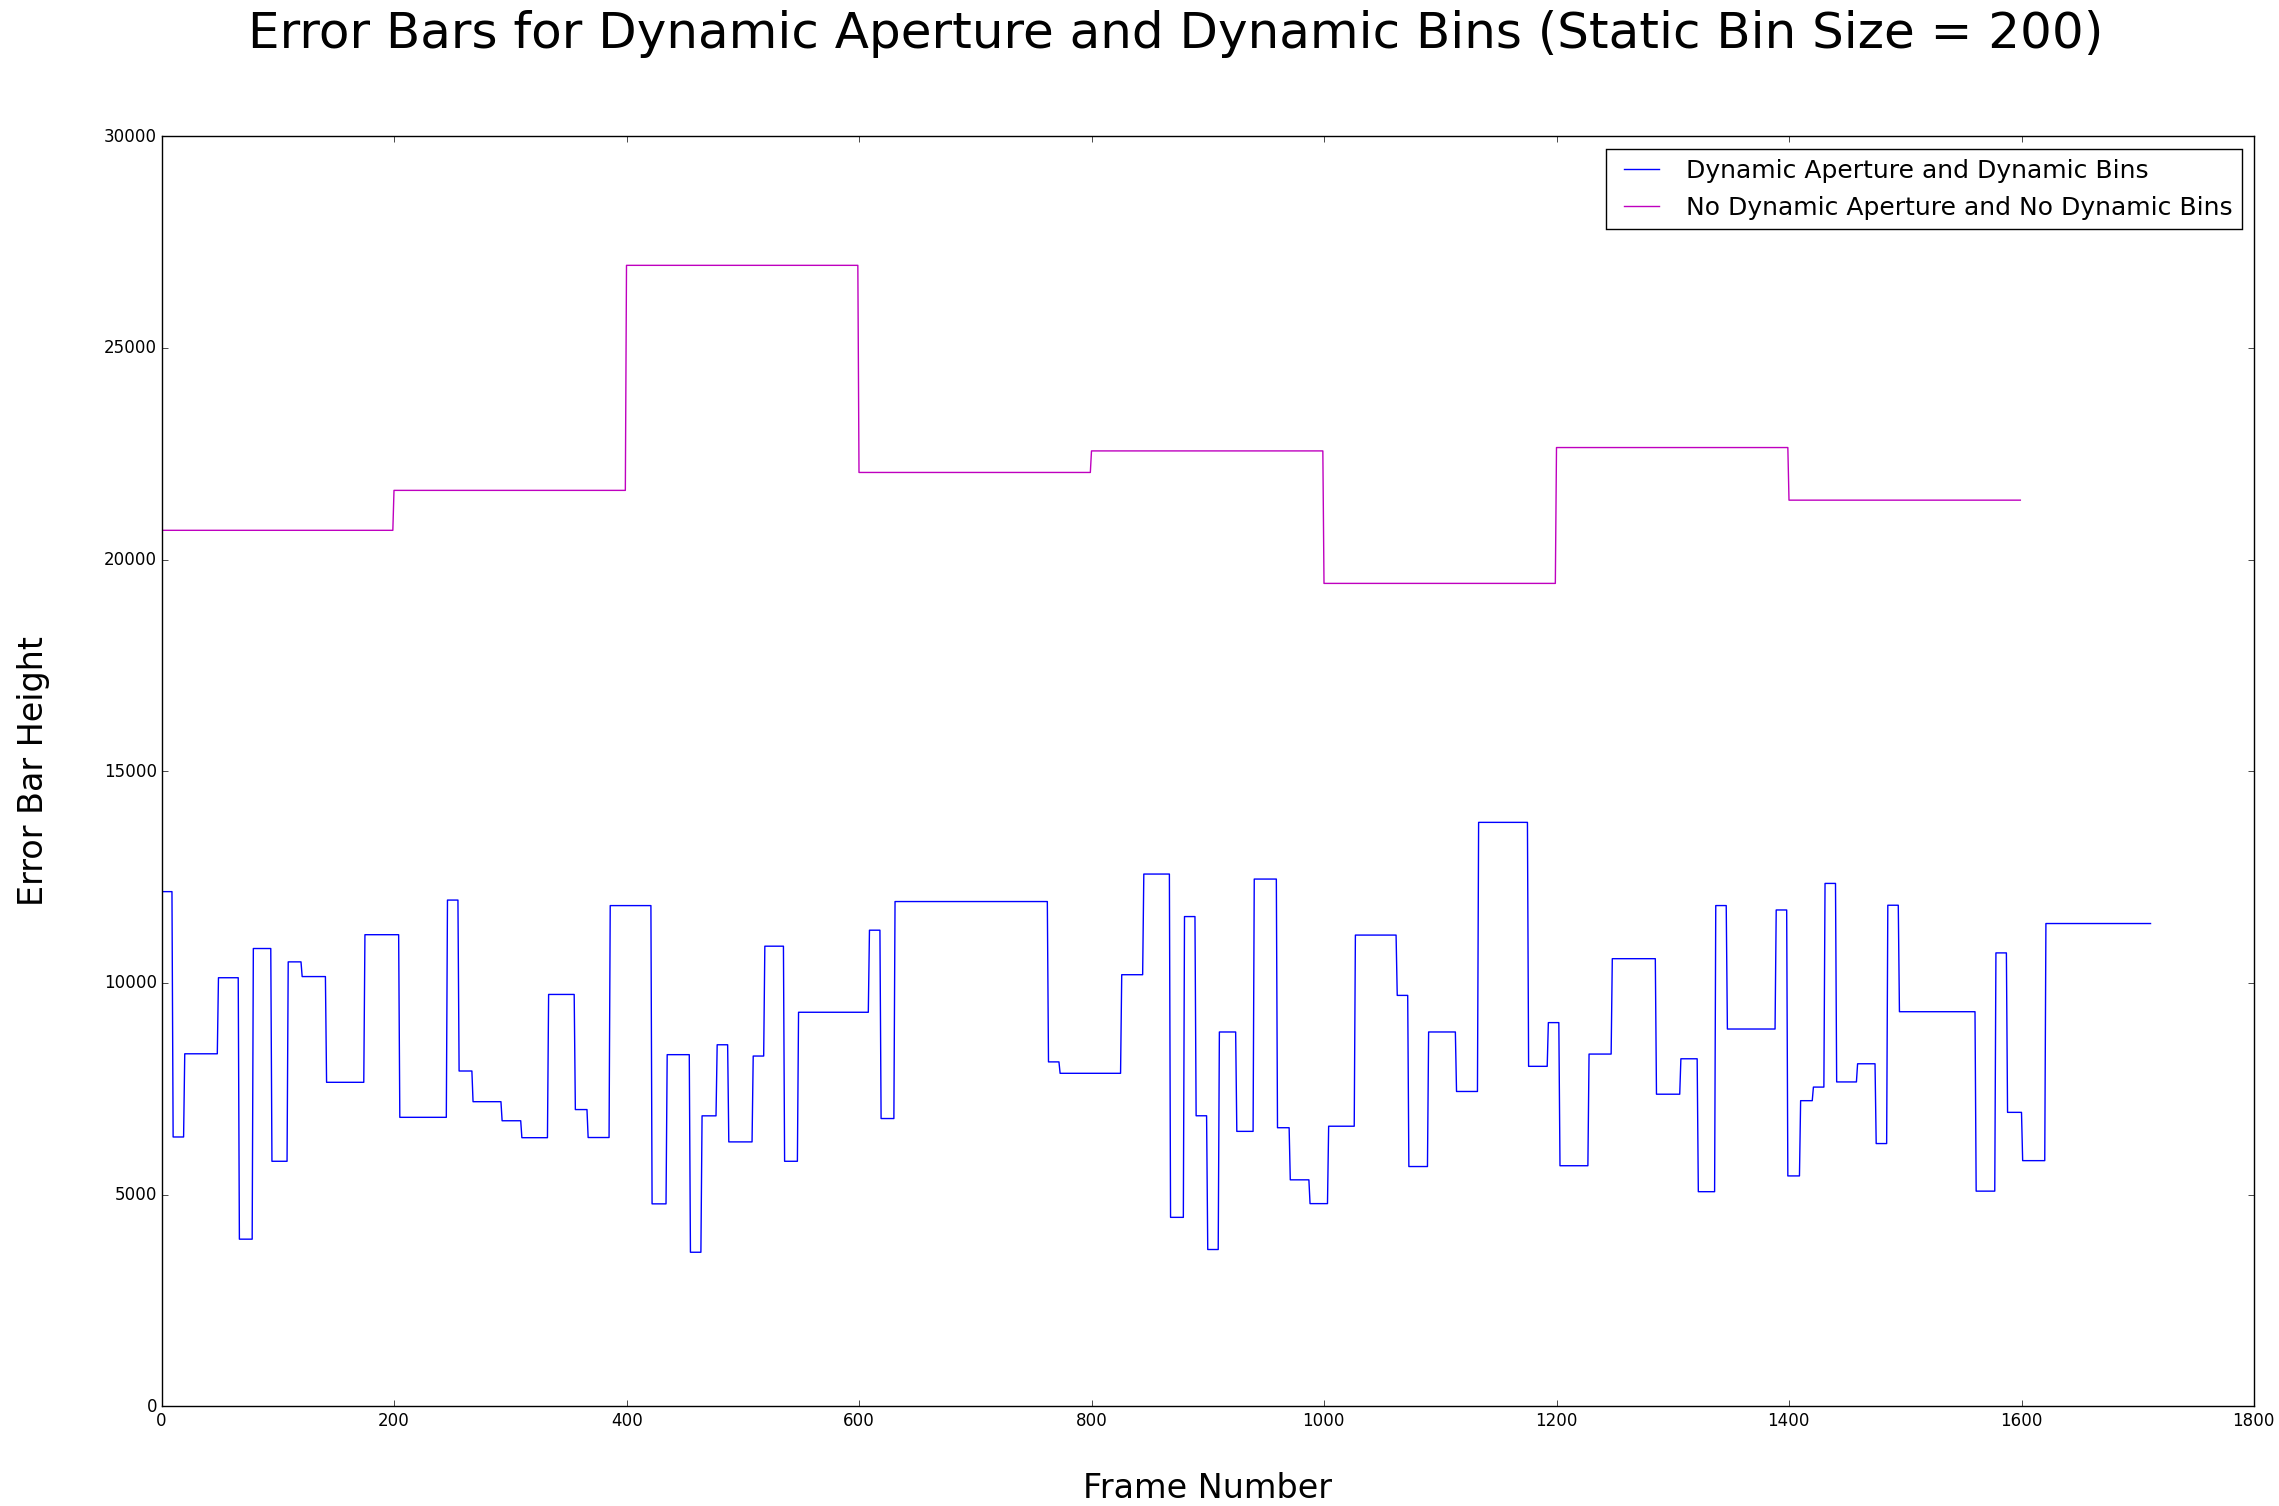
\includegraphics[scale = 0.3]{200.png}
\caption{Dynamic Aperture and Dynamic Blocking alongside neither. The Static Bin Size is 200.}
\end{center}
\end{figure}
\section{Conclusion}
\indent \indent These statistics and graphs all show the merit of using Dynamic Aperture and Dynamic Bins. The performance of these algorithms rests on a good choice of their parameters. For Dynamic Aperture, there is one parameter to tweak: the P-value. Too small a P-value can cut out the dimmest pixels in a star, making our intensities too low. Meanwhile, the error bars will be fantastically small. Too large a P-value will accurately sum up \textit{all} of the star with complete certainty, but may include more pixels as a result and hence a larger error bar. Dynamic Binning introduces two more variables: the maximum acceptable P-value and the maximum bin size. The maximum bin size is mostly a convenience of speeding up the program - the bins tend to stay closer to the lower limit induced by the maximum P-value of a measurement lying outside the error bar than by a maximum number of frames. This second parameter has a substantial impact on the output, quantitatively dictating how much advantage should be taken of small regions with low errors. Reasonable values of it are generally somewhere between 0.05 and 0.2, though of course circumstance should have the final say on how tolerant of mistakes we ought to be. All in all, though, irrespective of how immaculate a job we do of choosing our parameters fastidiously, Dynamic Aperture and Dynamic Bins allow for lower uncertainties in lightcurves, finer detail in fluctuations, and a better chance of detecting changes in source brightness, all at very little computational cost.
\end{document}